\section{Introduction}

\subsection{Background and Problem Definition}

Lectures as video materials for study in universities, online Courses, and professional Training are quite frequent. In addition, it is also inconvenient for efficient review at present. After returning from class, most of the time, students will no longer try to watch it all over again. Generally, there needs to be selection for definitions; determining whether an explanation of that concept is valid; making comparisons with similar Concepts; asking overly specific questions. Normal video players cannot meet the needs of such uses well. Mainly support linear playback and rough time-based navigation; they cannot meet the demand of technical lectures well.

Based on this, the research question of this paper is as follows: Given a raw lecture video, how do we make it more conducive to revisiting and posing questions? It does not need only to produce the abstract. We will combine three different concepts at a time.

\begin{itemize}
\item the \textit{temporal level}, where the system identifies meaningful lecture boundaries;
\item the \textit{semantic level}, where the content is converted into explicit knowledge units;
\item the \textit{interactive level}, where users can query the lecture and obtain grounded answers.
\end{itemize}

Not every conversion will be simple in practice. Lecture audio is usually noisy; there are no synchronised slide-up slides when the content changes; The instructor spends more than a minute explaining an idea without breaking it down clearly. Due to this reason, it is necessary for the system to have reasonable multi-modal segmentation as well as a grounding-based question-answering module during lectures.

\subsection{Method Overview}

LectureMind, as a multiple-stage architecture for understanding the content of lecture videos. Starting with simple audio/visual analysis of speeches and texts, it then integrates these two sets of data into a relatively close form of teaching unit compared with direct time segmentation. Then each part of the whole becomes more detailed knowledge point, which is organised as summary together with mind map-style organisation in turn. On top of these representations, we support three question answering modes: direct answering without retrieval, single-pass retrieval-augmented generation, and agentic multi-step retrieval.

Figure~\ref{fig:system-overview} summarizes this end-to-end transformation from raw video input to interactive educational output.

\begin{figure}[H]
    \centering
    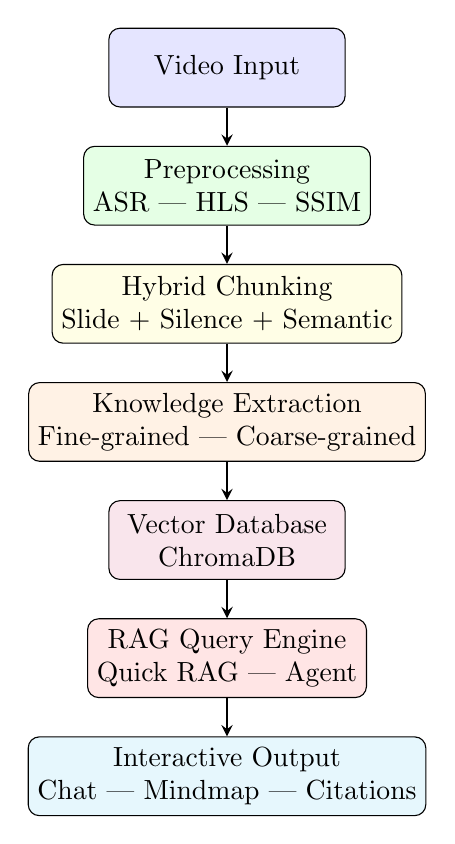
\begin{tikzpicture}[
        node distance=1.5cm,
        box/.style={rectangle, draw, rounded corners, minimum width=3cm, minimum height=1cm, align=center},
        arrow/.style={->, >=stealth, thick}
    ]
        \node[box, fill=blue!10] (input) {Video Input};
        \node[box, fill=green!10, below of=input] (preprocess) {Preprocessing\\ASR | HLS | SSIM};
        \node[box, fill=yellow!10, below of=preprocess] (chunking) {Hybrid Chunking\\Slide + Silence + Semantic};
        \node[box, fill=orange!10, below of=chunking] (knowledge) {Knowledge Extraction\\Fine-grained | Coarse-grained};
        \node[box, fill=purple!10, below of=knowledge] (storage) {Vector Database\\ChromaDB};
        \node[box, fill=red!10, below of=storage] (query) {RAG Query Engine\\Quick RAG | Agent};
        \node[box, fill=cyan!10, below of=query] (output) {Interactive Output\\Chat | Mindmap | Citations};

        \draw[arrow] (input) -- (preprocess);
        \draw[arrow] (preprocess) -- (chunking);
        \draw[arrow] (chunking) -- (knowledge);
        \draw[arrow] (knowledge) -- (storage);
        \draw[arrow] (storage) -- (query);
        \draw[arrow] (query) -- (output);
    \end{tikzpicture}
    \caption{LectureMind System Architecture Overview}
    \label{fig:system-overview}
\end{figure}

The main idea behind the framework is fairly simple: lecture understanding works better when the representation is hierarchical. Instead of treating the whole video as one long document, we break it into segments, map each segment to explicit knowledge, and organize those results into units that are small enough for retrieval but still meaningful on their own. That gives the QA system something more useful than isolated transcript sentences, while still keeping a clear link back to the original video.

\subsection{Contributions}

The following are the main outcomes or results achieved by this paper:

\begin{itemize}
\item An end-to-end approach to converting lecture videos into structured learning materials, including video Segmentation, knowledge Extraction and Grounded Question Answering.
\item We propose a combination of sliding window and boundary cue strategies for chunking to enhance the stability when using only one signal.
\item We propose a three-mode retrieval-aided answering architecture based on the balancing of reasoning depth, response speed and answer credibility via cascade fallback strategies.
\end{itemize}
